\section{Ray tracing}

Ray tracing involves considering the light emitted by other objects in two distinct directions: mirror reflection and refraction for transparent objects. 
This is mathematically represented as follows:
\begin{multline*}
    L(x,\omega_r)=L_e(x,\omega_r)+\sum_l L(l,\overrightarrow{lx})f_{r}(x,\overrightarrow{lx},\omega_r)V(x,l)+L(r,\overrightarrow{rx})f_{r^{\prime}}(x,\overrightarrow{rx},\omega_r)V(x,r)+\\+L(t,\overrightarrow{tx^\prime})f_{t^\prime}(x^\prime,\overrightarrow{tx^\prime},\omega_r)V(x,t)
\end{multline*}
In this equation, $L(x,\omega_r)$ represents the radiance at point $x$ in direction $\omega_r$. 
The first term $L_e(x,\omega_r)$ accounts for emitted radiance. 
The summation term involves contributions from other objects: $L(l,\overrightarrow{lx})$ denotes radiance from objects in the scene, $f_{r}(x,\overrightarrow{lx},\omega_r)$ represents the reflection function for mirror reflection, $f_{r^{\prime}}(x,\overrightarrow{rx},\omega_r)$ accounts for mirror reflection, and $f_{t^\prime}(x^\prime,\overrightarrow{tx^\prime},\omega_r)$ represents the refraction function. 
$V(x,l)$, $V(x,r)$, and $V(x,t)$ are visibility functions indicating whether the light from a given direction is visible from the viewpoint.
In this equation, the second term of the summation handles mirror reflection, while the third term considers refraction.

\paragraph*{Reflection}
In the context of reflection, this direction corresponds to the mirror direction: the angle of reflection equals the angle of incidence but on the opposite side relative to the surface normal at the point of impact. 
This facilitates the recreation of realistic perfect (mirror-like) reflections. Specifically, at each point $x$, the algorithm searches for points $r$ on all objects within the scene along the mirror direction $\overrightarrow{rx}$ and chooses the one closest to $x$.

\paragraph*{Refraction}
In the context of refraction, the algorithm emulates the physical properties of objects by incorporating the material's index of refraction to determine the angle of the refracted ray. 
Here, for each point $x$, the algorithm initially identifies the exit point $x^\prime$ from which the ray will on the opposing side by considering the varying refractive indices of the materials separated by the surface.
Subsequently, it searches for points $t$ on all objects along the direction $\overrightarrow{tx}^\prime$. 

\paragraph*{Ray casting}
The algorithm relies on a ray-casting procedure to determine the colors visible from a given point in space $x$ and direction $\omega$.
This procedure identifies the closest object to point $y$ in the specified direction $\omega$ and utilizes the approximated rendering equation to compute $L(y,\omega)$.
Initially, the algorithm iterates over each point on the projection plane (each pixel of the generated image) in the direction of the projection ray, applying the ray-casting procedure to each.

To incorporate reflection and refraction into each pixel, the procedure is invoked recursively with the computed points and directions. 
This recursion continues up to a defined number of bounces, known as the ray depth.

Light sources remain distinct from objects, and visibility for light sources is also accounted for. 
In this case, ray tracing determines whether a light source is visible or not.
This determination is made by the first term of the summation. 
If the reflected ray does not intersect with any other object in the direction of the light, then the light source is considered visible. 
However, if the ray intersects with another object, the light is deemed obstructed and excluded from the rendering equation.

\subsection{Ray-tracing pipeline}
Frameworks such as Vulkan and DirectX offer dedicated pipelines to facilitate real-time ray tracing, provided that compatible GPUs are accessible. 
In Vulkan, this pipeline is referred to as the Ray Tracing pipeline.
\begin{figure}[H]
    \centering
    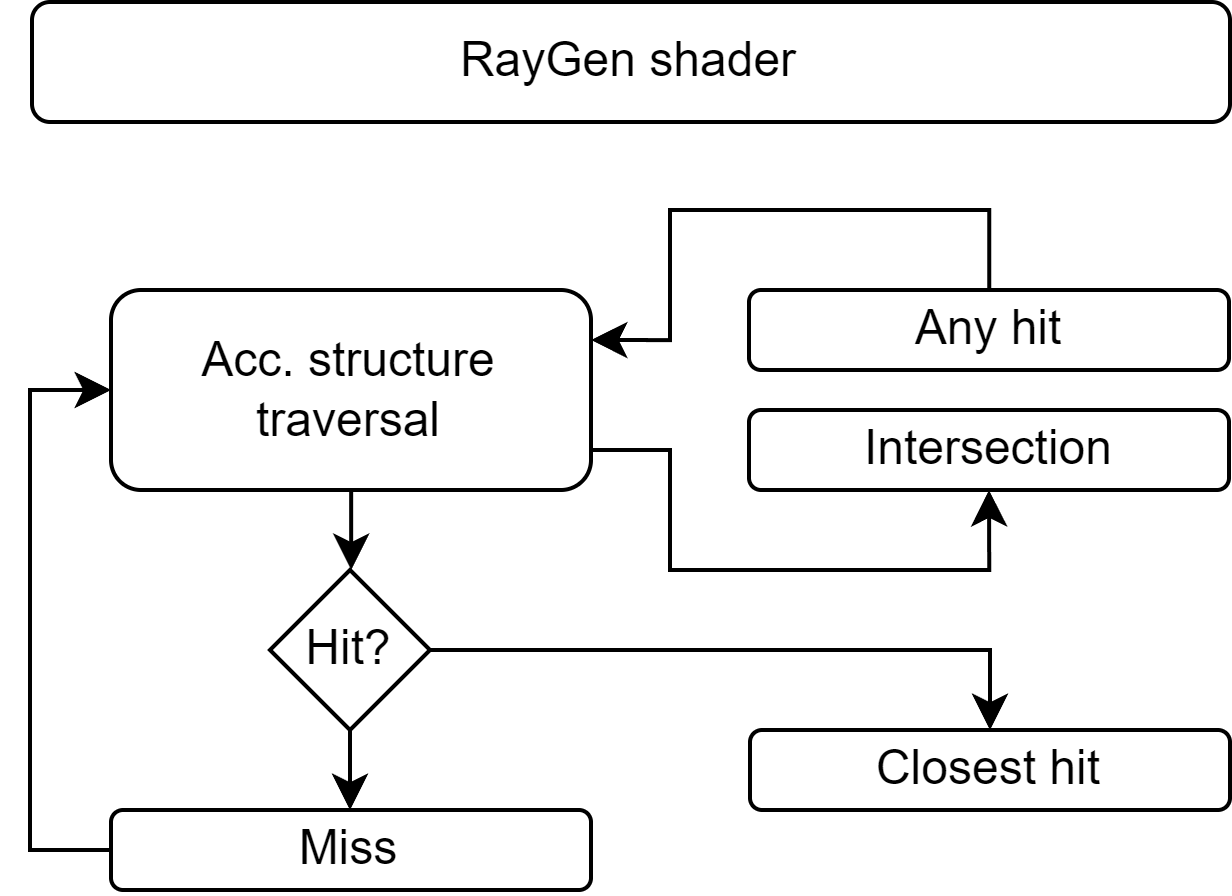
\includegraphics[width=1\linewidth]{images/rayt.png}
    \caption{Shaders}
\end{figure}
The ray-tracing pipeline generates images by casting rays from the pixels on the screen, unlike the traditional graphics pipeline driven by triangles and vertices. 
For each fragment on the screen, a ray is projected into the scene and intersects with all the triangles of all the meshes in the 3D environment. 
Only the closest intersection to the viewer is considered.

To compute the color of each fragment accurately, additional rays are traced to reproduce reflections and refractions (transparencies). 
In the presented ray-tracing rendering technique, these rays typically include the perfect reflection ray, the refraction ray, and the rays connecting the point to the light sources.

Determining intersections with all triangles in the scene is a computationally intensive task. 
Without proper optimization, it can have a complexity of $O(n)$ in the number of triangles. 
Special acceleration structures provided by the user are necessary to address this complexity. 
Due to time constraints, a detailed discussion of these structures cannot be provided here.

The ray-tracing pipeline requires five shaders to compute and handle all triangle-ray intersections.

\paragraph*{RayGen shader}
The RayGen shader is executed for each output fragment of the images, responsible for determining the starting point and direction of the corresponding ray in the scene. 
Typically, it considers each pixel on the screen and casts a ray from the camera's viewpoint in the corresponding direction.

However, users are not limited to considering a planar projection plane with equally-spaced pixels. 
Cylindrical and spherical projections can be easily implemented with minor adjustments to the RayGen procedure.

\paragraph*{Intersection and closest hit}
The intersection shader enables the implementation of custom ray-triangle intersection procedures. 
On the other hand, the closest hit shader is invoked on the point closest to the viewer. 
Its primary function is to compute the color of the point by approximating the rendering equation, akin to a fragment shader in the graphics pipeline.
Additionally, it can recursively cast other rays to handle effects like reflections and refractions.

\paragraph*{Any hit and miss}
The any hit shader serves to filter out intersections that should not be considered, such as those involving partially transparent objects. 
It provides a mechanism to handle such cases effectively.

On the other hand, the miss shader is invoked when the ray does not hit any object in the scene. 
Typically, it is utilized to render a background that appears behind all other objects in the scene.

\paragraph*{Structure traversal}
The fixed part of the ray-tracing pipeline governs the traversal of acceleration structures and the determination of the closest hit. 
While this approach is powerful, it demands significant computational resources. 
Only the most advanced GPUs available today can provide satisfactory performance for real-time ray tracing.

\subsection{Algorithm}
The pseudo-code of a ray tracing rendering algorithm is the following:
\begin{algorithm}[H]
    \caption{Ray tracing rendering algorithm}
        \begin{algorithmic}[1]
            \For{each pixel $x$ on screen}
                \State{Compute color casting a ray from $x$ according the projection}
            \EndFor{}
        \end{algorithmic}
\end{algorithm}
The ray-casting procedure is the heart of the technique:
\begin{algorithm}[H]
    \caption{Ray casting procedure}
        \begin{algorithmic}[1]
            \State{Determine the point $q$ of the closest object with respect to the ray}
            \State{Set the pixel color $C = 0$}
            \For{each light $l$ in the scene}
                \If{light $l$ is not occluded (ray-casting)}
                    \State{Set $C = C + \text{contribution of light } l \text{ to } q$}
                \EndIf{}
            \EndFor{}
            \State{Set $C = C + \text{reflection contribution}$ (recursion)}
            \State{Set $C = C + \text{refraction contribution}$ (recursion)}
        \end{algorithmic}
\end{algorithm}
Indeed, the number of traced rays can potentially double at each step in ray tracing, leading to significantly increased rendering times. 
Additionally, it necessitates the computation of the closest intersection using acceleration structures instead of relying on the Z-buffer, as in traditional rasterization techniques.

Ray tracing offers the capability to incorporate mirror reflection and transparency with refraction. 
This enables realistic rendering of materials such as glass, fluids, and shiny metals, among others.

However, it's important to note that ray tracing has limitations. 
It is not inherently capable of simulating indirect lighting or handling glossy reflections, which restricts the level of realism achievable with this technique.